\section{Résultats}

\begin{minipage}{\textwidth}
    \begin{wrapfigure}{R}{0.55\textwidth}
        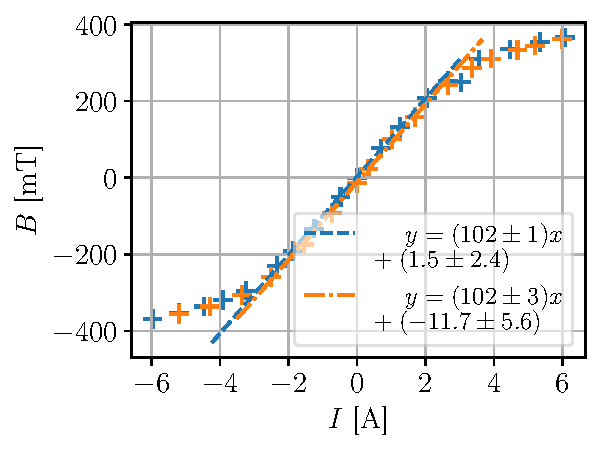
\includegraphics[width=\linewidth]{figures/calibration.pdf}
        \caption{Variation de l'amplitude du champ magnétique en fonction du courant sur un cycle \(I_\textrm{max} \rightarrow 0 \rightarrow -I_\textrm{max} \rightarrow 0 \rightarrow I_\textrm{max}\).}
        \label{fig:callibration}
    \end{wrapfigure}

    \paragraph*{Étalonnage du champ d'induction}
    La \autoref{fig:callibration} montre comment varie le champ magnétique en fonction du courant. Ici, \(I_\textrm{max} = 6\) \si{\ampere}. Par souci de clarté, les erreurs sur les mesures ne sont pas affichées dans cette figure et sont de l'ordre de 2\%. Les points bleus correspondent à la partie descendante du cycle et les points oranges à la partie montante. Deux fit linéaire on été réalisés sur la partie linéaire (entre -3 \si{\ampere} et 3 \si{\ampere}), 1 pour chaque sens, et mettent en évidence une légère hystérèse, puisque les deux droites sont décalées, d'ordonnée à l'origine \(\beta_1 = (1.5 \pm 2.4)\) pour la partie descendante contre \(\beta_2 = (-11.7 \pm 5.6)\) pour la partie montante.

    \paragraph*{Mesure des tensions résiduelles pour InP}
    Blabla regarde tension résiduelle pour un courant nul \autoref{tab:tension_residuelle}
    % Mettre le début de ce paragraphe dans la minipage puis sortir pour esquiver la légende de la figure...
\end{minipage}

% Suite du paragraphe tensions résiduelles

\begin{table}[h]
    \centering
    \begin{tabulary}{\textwidth}{C C C C}
        \toprule
        Configuration \si{\micro\meter} & Tension (\(a = 1\) \si{\micro\meter}) [\si{\milli\volt}] & Tension (\(a = 2\) \si{\micro\meter}) [\si{\milli\volt}] \\
        \midrule
        \(I_{13}U_{24}\) & \(68.74 \pm 0.01\) & \(27.02 \pm 0.01\) \\
        \(I_{31}U_{42}\) & \(68.69 \pm 0.01\) & \(27.12 \pm 0.01\) \\
        \(I_{24}U_{13}\) & \(39.93 \pm 0.01\) & \(24.78 \pm 0.01\) \\
        \(I_{42}U_{31}\) & \(40.12 \pm 0.01\) & \(24.76 \pm 0.01\) \\
        \bottomrule
    \end{tabulary}
    \caption{Tension résiduelle pour différentes configuration et 2 épaisseurs de l'échantillon InP}
    \label{tab:tension_residuelle}
\end{table}

\paragraph*{Détermination de la constante de Hall pour InP}
Regarde ces belles relations linéaires uwu

On trouve pour 1µm \(R_H = (2.40 \pm 0.05) \cdot 10^{-3}\) \si{\meter\cubed\per\coulomb} et \(N = (2.60 \pm 0.05) \cdot 10^{21}\) \si{\per\meter\cubed}

On trouve pour 2µm \(R_H = (1.47 \pm 0.03) \cdot 10^{-3}\) \si{\meter\cubed\per\coulomb} et \(N = (4.25 \pm 0.08) \cdot 10^{21}\) \si{\per\meter\cubed}

\begin{figure}[h]
    \centering
    \begin{subfigure}{0.45\textwidth}
        \centering
        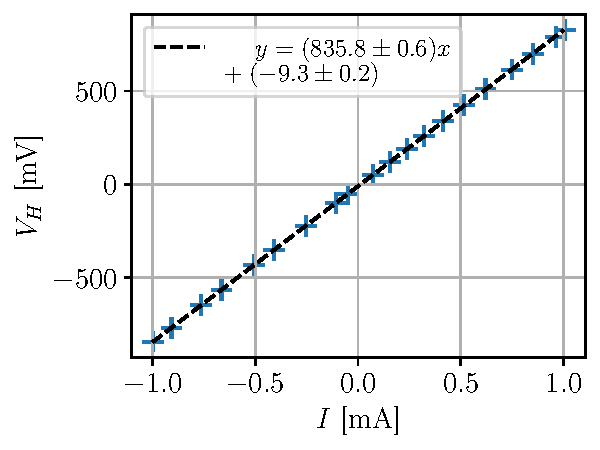
\includegraphics[width=\textwidth]{figures/U(I),InP1micro.pdf}
        \caption{}
    \end{subfigure}
    \begin{subfigure}{0.45\textwidth}
        \centering
        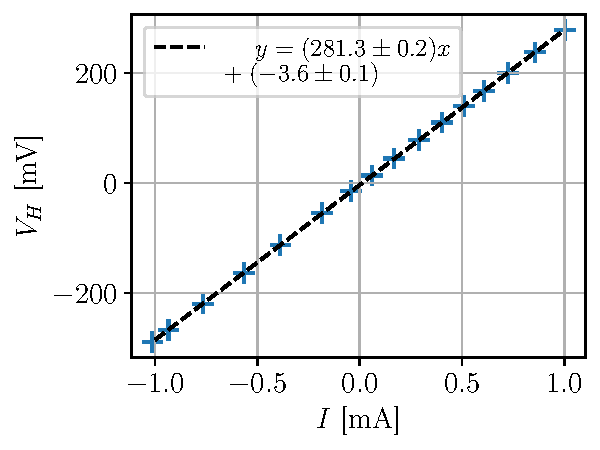
\includegraphics[width=\textwidth]{figures/U(I),InP2micro.pdf}
        \caption{}
    \end{subfigure}
    \caption{Tension en fonction de l'intensité pour l'échantillon InP d'épaisseur (a) 1 \si{\micro\meter} (b) 2 \si{\micro\meter}}
\end{figure}

\begin{figure}[h]
    \centering
    \begin{subfigure}{0.45\textwidth}
        \centering
        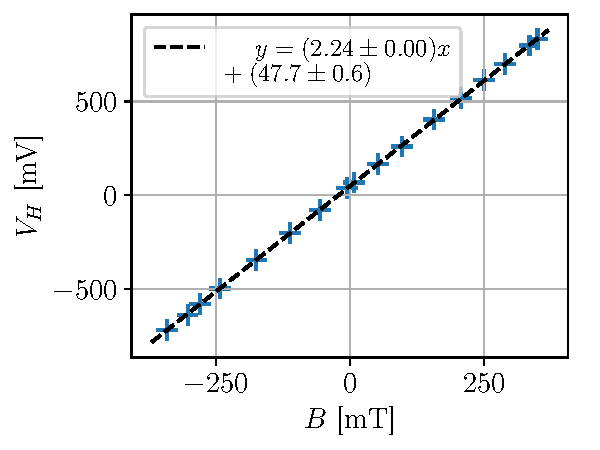
\includegraphics[width=\textwidth]{figures/U(B),InP1micro.pdf}
        \caption{}
    \end{subfigure}
    \begin{subfigure}{0.45\textwidth}
        \centering
        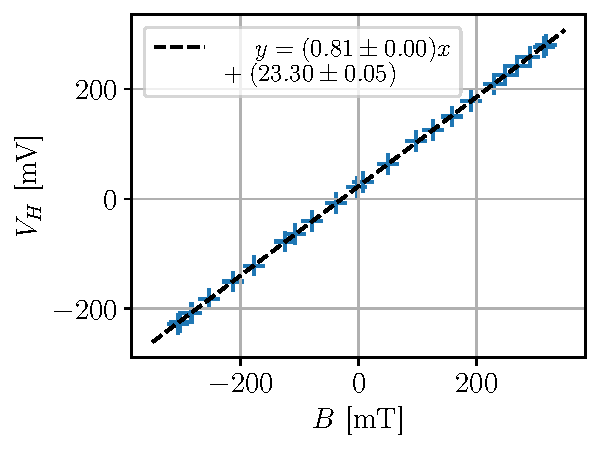
\includegraphics[width=\textwidth]{figures/U(B),InP2micro.pdf}
        \caption{}
    \end{subfigure}
    \caption{Tension en fonction de la norme signée du champ magnétique pour l'échantillon InP d'épaisseur (a) 1 \si{\micro\meter} (b) 2 \si{\micro\meter}}
\end{figure}
